\documentclass[preprint,12pt]{elsarticle}

    \usepackage[sc]{mathpazo} % Use the Palatino font
    \usepackage[T1]{fontenc} % Use 8-bit encoding that has 256 glyphs
    \usepackage{microtype} % Slightly tweak font spacing for aesthetics
    \usepackage[english]{babel} % Language hyphenation and typographical rules
    \usepackage{booktabs} % Horizontal rules in tables
    \usepackage{enumitem} % Customized lists
    \usepackage[table,xcdraw]{xcolor}
    \usepackage[utf8]{inputenc} % Required for inputting international characters
    \usepackage{parskip}
    \usepackage{graphicx}
    \usepackage{hyperref}
    \usepackage{pdfpages}
    \usepackage{amsmath}
    \usepackage{esvect}
    \usepackage{listings}
    \usepackage[title]{appendix}
    \hypersetup{
        colorlinks=true,
        linkcolor=blue,
        filecolor=magenta,      
        urlcolor=cyan,
    }
    
    \begin{document}
    \begin{frontmatter}
    \title{\LARGE \bf
        MNIST Handwriting Recognition
        }
        
        \author{ \parbox{3 in}{\centering Chongyi Xu \\
                 University of Washington\\
                 AMATH 482/582 Winter Quarter 2018\\
                 {\tt\small chongyix@uw.edu}}
        }

    
    \begin{abstract}
        For this project, we will use MNIST handwritten digit dataset to build neural networks, which might
        help us as a detector of digits. MNIST database has 60000 images of handwriting digits with labels 
        as training data and another 10000 images also with labels as testing data. A single layer and a 
        2 layer will be programmed to classify each digit.
    \end{abstract}
    \end{frontmatter}
    
    \section{Introduction and Overview}
        Neural networks (NNs)are computing systems vaguely inspired by the biological neural networks 
        that constitute animal brains. Such systems "learn" (i.e. progressively improve performance on) 
        tasks by considering examples, generally without task-specific programming. For example, in 
        image recognition, they might learn to identify images that contain cats by analyzing example
        images that have been manually labeled as "cat" or "no cat" and using the results to identify 
        cats in other images. They do this without any a priori knowledge about cats, e.g., that they
        have fur, tails, whiskers and cat-like faces. Instead, they evolve their own set of relevant
        characteristics from the learning material that they process.
    
    
        %------------------------------------------------
        \section{Theoretical Background}
        Consider we have an input spike $\mathbf{x}$, we would like to know if input object is either a dog or a cat.
        Neural network says that, with a series of mapping function $f$, we would find a mapped perceptron $\mathbf{y}$
        such that we could make our decision based on the output value of the perceptron, for instance, $ 1 = dog$ and 
        $-1 = cat$. During the training process, we would like to get such $f$ for our network, from the data matrix.
        For example, we have 5 dogs(A, B, C, D, E) and 5 cats(a, b, c, d, e), the training process is as simple as telling 
        the machine that A~E are dogs and a~e are cats.
        \begin{equation*}
            [1\ 1\ 1\ 1\ 1\ -1\ -1\ -1\ -1\ -1] = f([A\ B\ C\ D\ E\ a\ b\ c\ d\ e])
        \end{equation*}
        And the $f$ is what we are looking for. $f$ will differ with different layers. In this project, I will focus on 
        a single-layer network and a 10-layer networks as an example of multi-layer networks.  
    
        \subsection{One Layer Network}
        \begin{figure}[h]
            \center
            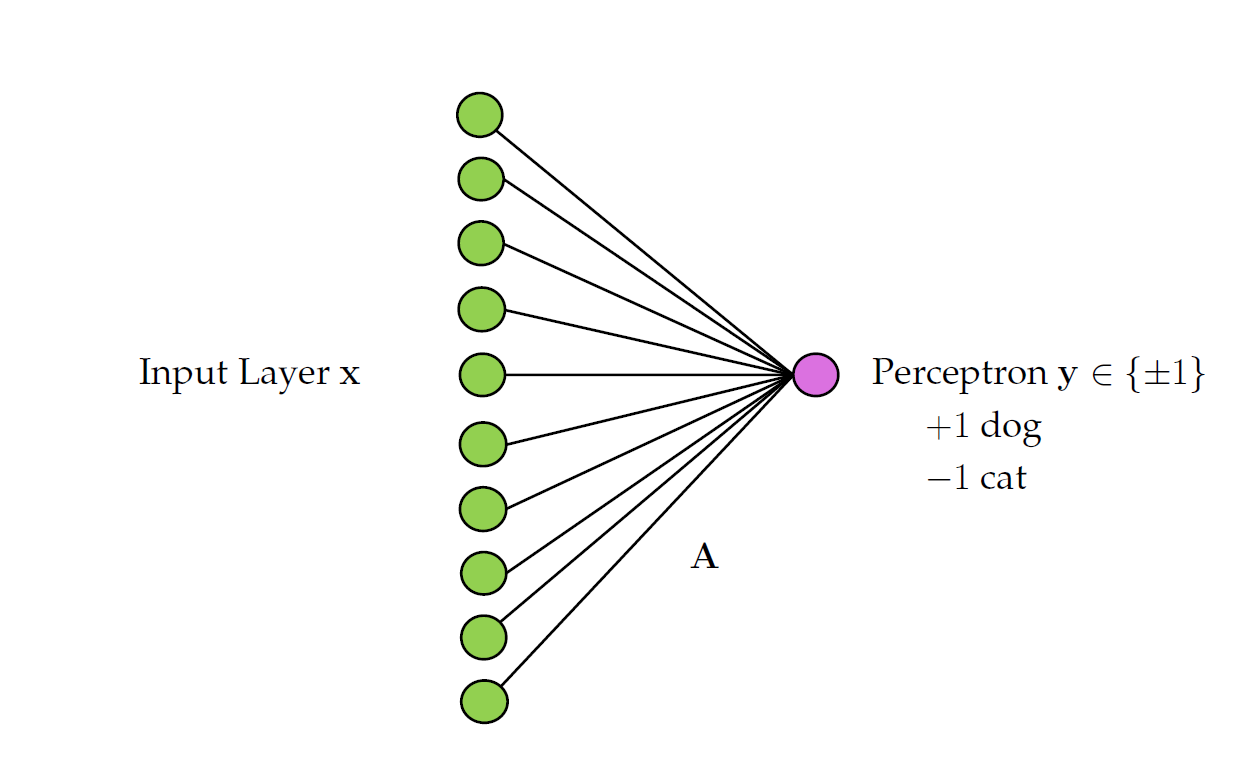
\includegraphics[width = 0.8\textwidth]{onelay.PNG}
            \caption{Single Layer Network}
            \label{fig:1}
        \end{figure}
        With one layer, as shown in the Figure \ref{fig:1}, it will classify the object after one single linear map and 
        give the decision based on the output of the perceptron.
        \begin{equation*}
            \mathbf{Y} = A \mathbf{X}
        \end{equation*}
        And the layer $A$ could be simply calculated by 
        \begin{equation*}
            A = \mathbf{Y} \mathbf{X}^{+}
        \end{equation*}
        This gives a least-square regression for the mapping matrix $A$.
    
        \subsection{Multiple Layer Networks}
        As for some more complicated mapping models, like what we as humans always do, it is needed to have a higher-order
        layer for making decision.
        \begin{figure}[h]
            \center
            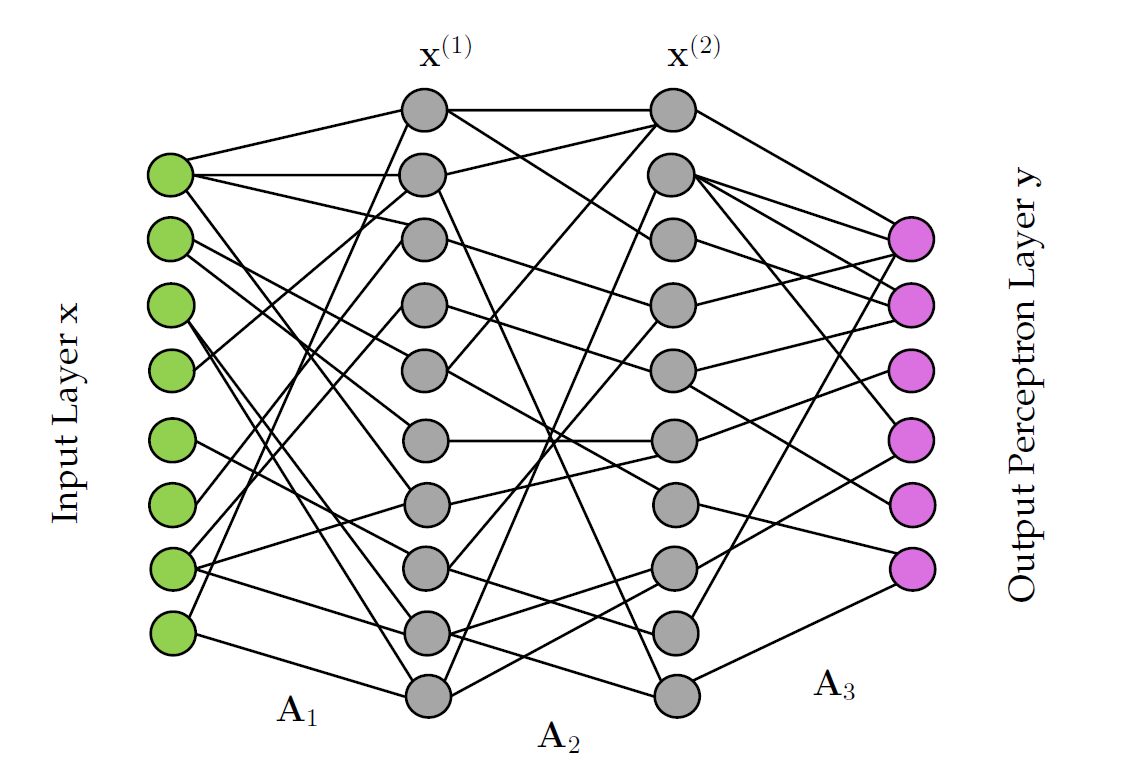
\includegraphics[width = 0.8\textwidth]{arc.PNG}
            \caption{Two Layer Network}
            \label{fig:2}
        \end{figure}
        Figure \ref{fig:2} is an example of two-layer net architecture. It can be seen that the mapping process now becomes
        much more complicated rather than a single layer. 
        \begin{figure}[h]
            \center
            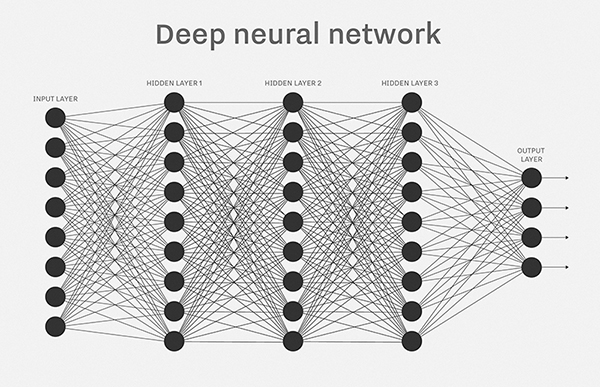
\includegraphics[width = 0.8\textwidth]{nn.jpg}
            \caption{Three Layer Network}
            \label{fig:3}
        \end{figure}
        Figure \ref{fig:3} shows how mapping goes to chaos as the number of layers get increased. And constructing such network is
        also known as deep learning process since the machine now is trying to learn by itself how to make decision. And 
        the training for N layer neural network to the data matrix X will be
        \begin{align*}
            \mathbf{X^{(1)}}    &= f_1(A_1, \mathbf{X}) \\
            \mathbf{X^{(2)}}    &= f_2(A_2, \mathbf{X^{(1)}}) \\
                                &\vdots \\
            \mathbf{X^{(N - 1)}}    &= f_N(A_{N-1}, \mathbf{X^{(N-2)}}) \\
            \mathbf{X^{(N)}}    &= f_N(A_N, \mathbf{X^{(N-1)}}) \\
            \mathbf{Y}          &= f_N(A_n, f_{N-1}(A_{N-1}, \dots f_1(A_1, \mathbf{X})))
        \end{align*}
        The mapping and remapping will repeat for N times until we get to the final layer, the output layer. And the $\mathbf{Y}$
        value will be the perceptron of the whole network.

        \section{Algorithm Implementation and Development}
        \subsection{Single Layer}
        For the single layer, I modified \href{https://github.com/synsis/SINGLE-LAYER-PERCEPTRON-for-MNIST}{synsis's work} to build
        a weight algorithm. The general algorithm is to find a weight $A_j$ such that for every pattern (in this project, $j\in [0, 9]$)
        the outer product of the pixel vector and the weight will generate the perceptron to detect the digit image.
        \begin{equation*}
            Y_{ij} = A_{ij} * X_{ij}, \textit{where } i = 1,\ 2,\ \dots N,\ j = 1,\ 2,\ \dots 10
        \end{equation*} 
        And for every training image, the training process will result in either 1 for correct detection or -1 for wrong detection. 
        The algorithm itself will have a learning rate at $\alpha = 0.1$ to know that if the weight is good or not. 
        
        \subsection{Two Layers}
        For the two-layer network, I basically used the same idea as I did in the single-layer network, but this time train the model
        use two weights, $w_{between}$ and $w_{output}$. 
        %------------------------------------------------
    
        \section{Computational Results}
        \subsection{Relearning Times}
        \begin{figure}[h]
            \center
            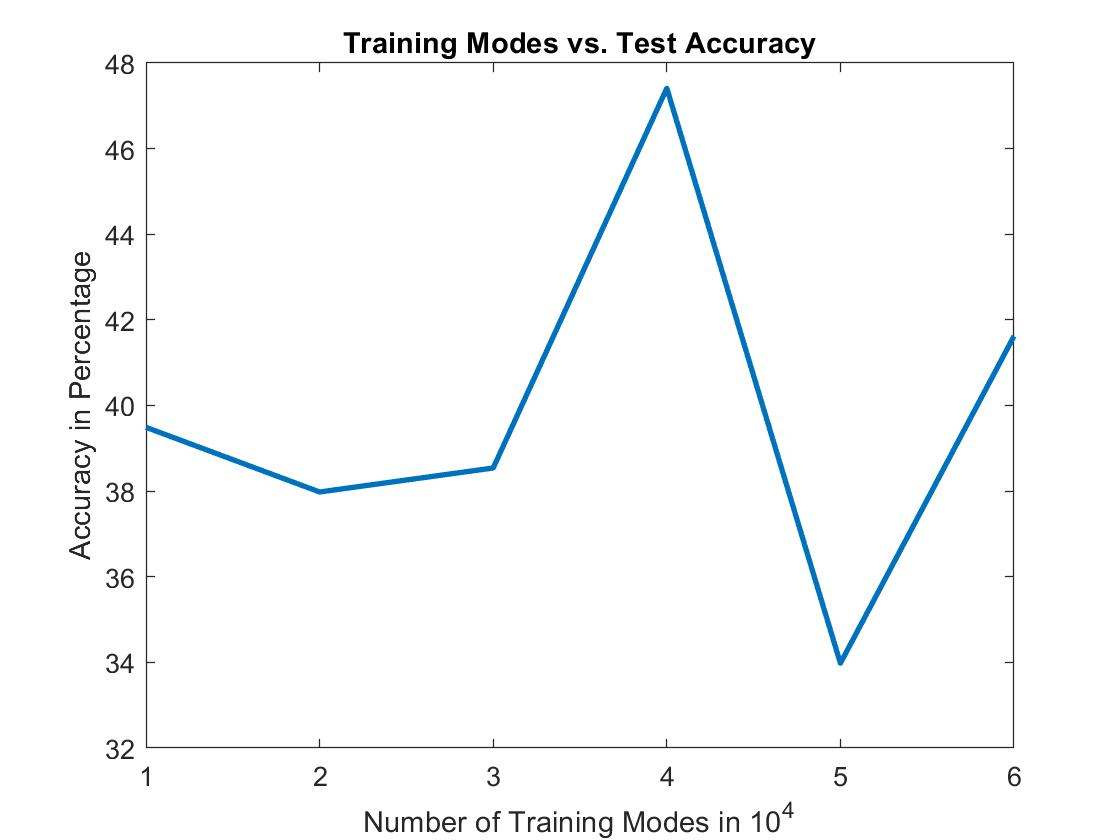
\includegraphics[width = 0.8\textwidth]{learn.jpg}
            \caption{Accuracy vs. Relearning times}
            \label{fig:4}
        \end{figure}
        Figure \ref{fig:4} shows how the accuracy changes as the relearning times increases.
        
        \subsection{Number of Epochs}
        \begin{figure}[h]
            \center
            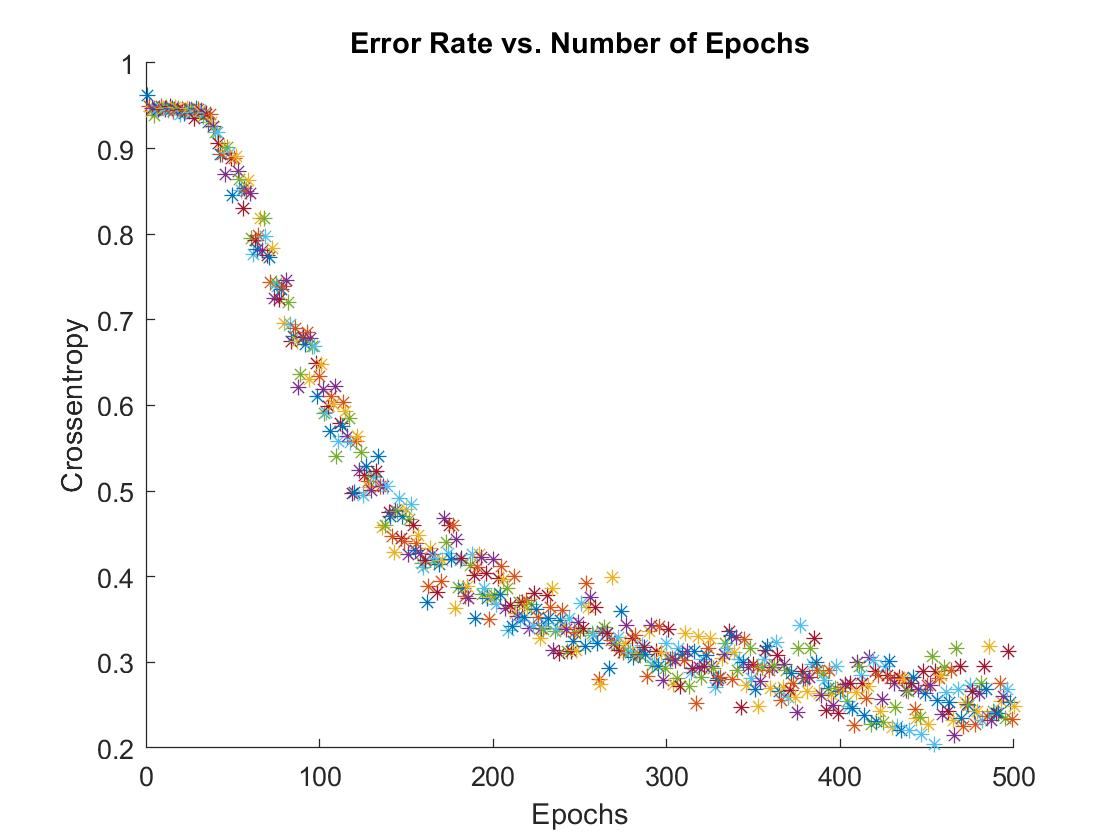
\includegraphics[width = 0.8\textwidth]{err.jpg}
            \caption{Performance of the network}
            \label{fig:5}
        \end{figure}
        Figure \ref{fig:5} shows how the error rate changes as the number of epochs increases.

        As the result, the accuracy of one single layer is about $39.84 \pm 0.2\%$ and the accuracy of two layers 
        is about $92\%$
        \begin{figure}[h]
            \center
            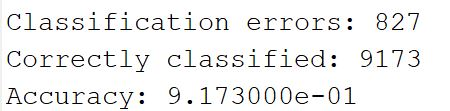
\includegraphics[width = 0.8\textwidth]{result.jpg}
            \caption{Result Output of Two-Layer Network}
            \label{fig:5}
        \end{figure}


        \section{Summary and Conclusion}
        As a conclusion, one single layer network does not perform well enough on detecting digits. A $~40\%$ accuracy
        is not considered to be reliable. Meanwhile, a two-layer network has much more better performance on the accuracy.

        %----------------------------------------------------------------------------------------
        %	APPENDIX
        %----------------------------------------------------------------------------------------
    
        \mbox{~}
        \clearpage
        \begin{appendices}
            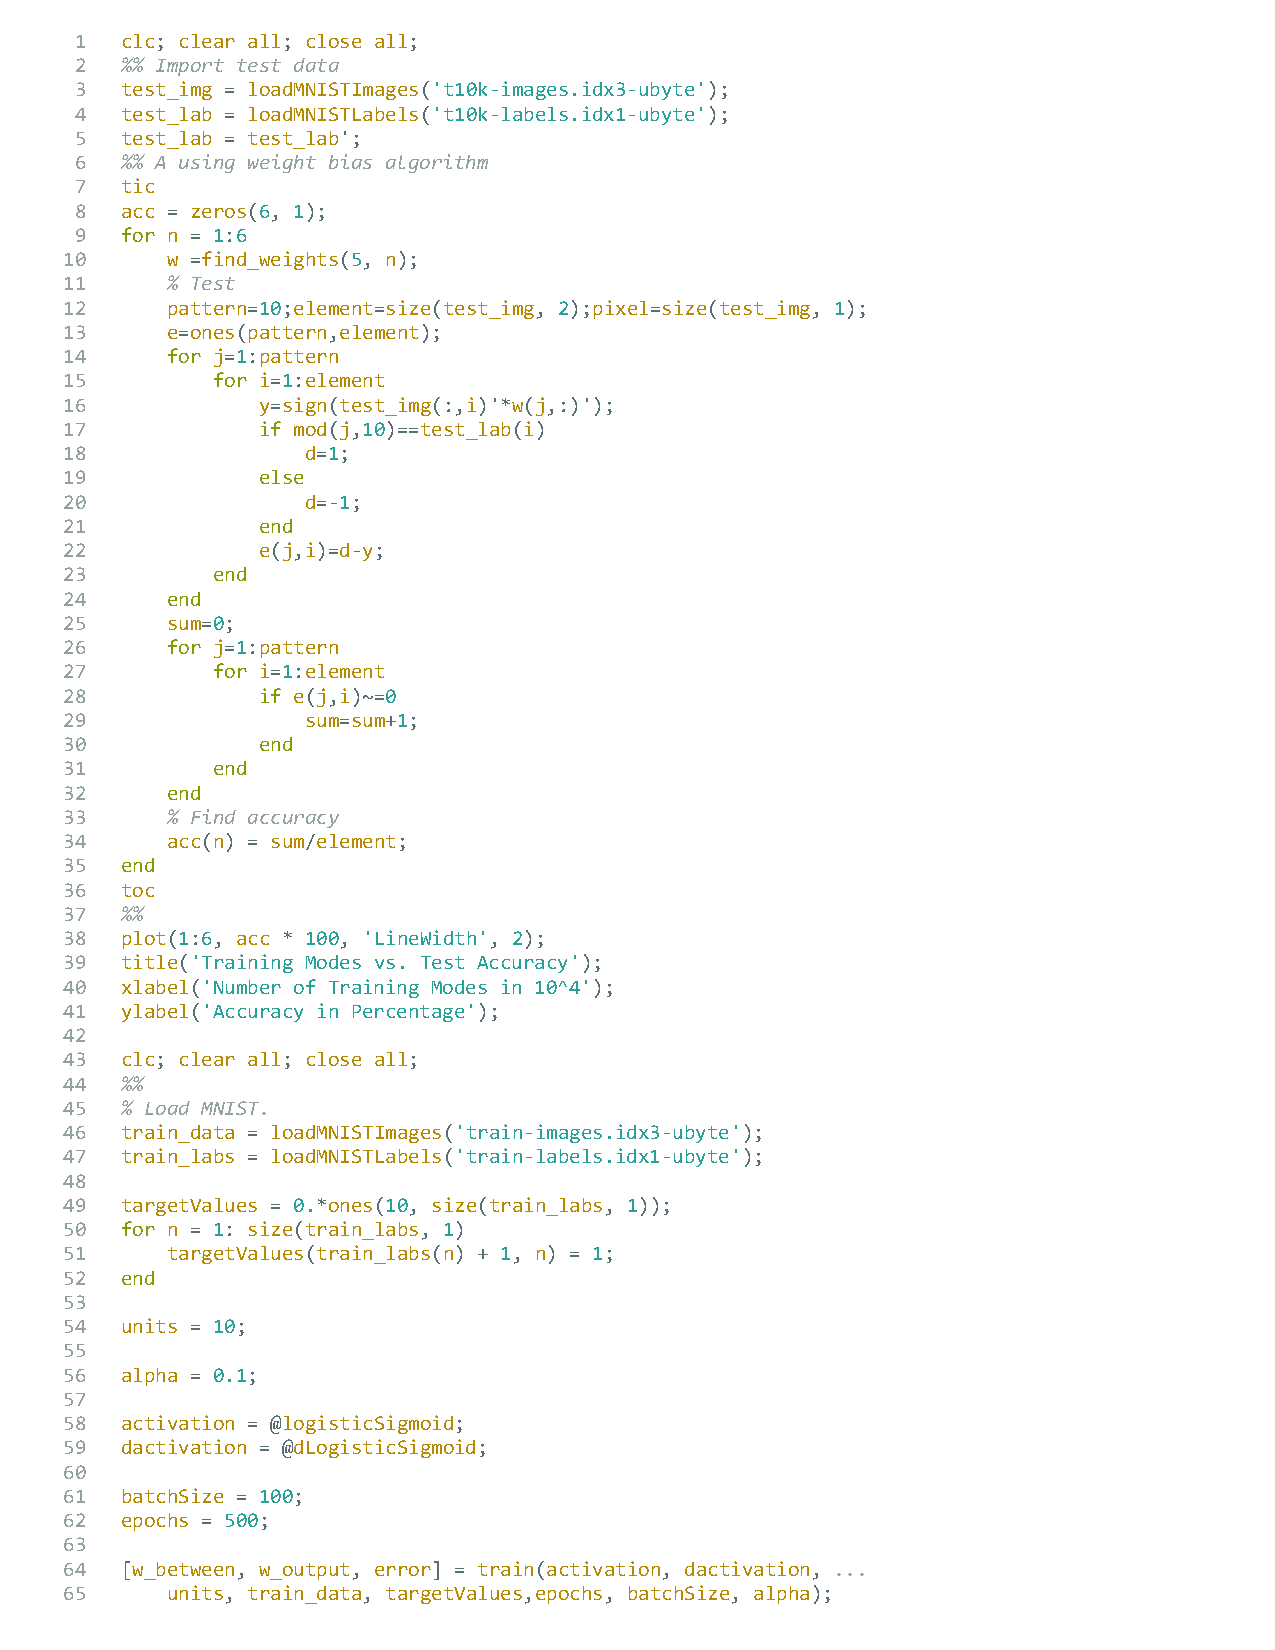
\includepdf[pages=-]{appendix.pdf}
        \end{appendices}
    
    \end{document}
    